\documentclass[a4paper,12pt]{article}

%% Standard
\usepackage[ngerman]{babel} 
\usepackage[utf8]{inputenc}
\usepackage[T1]{fontenc}

%% Mathe
\usepackage{amsmath}
\usepackage{amssymb}
\usepackage{amsthm}
\usepackage{latexsym}

%% Aufzaehlungen
\usepackage{enumerate}

%% Bilder
\usepackage{subfigure}
\usepackage{graphicx}

%% Absaetze usw
\usepackage{multicol}   
% zu verwenden mit 
% \begin{multicols}{$$Spaltenanzahl$$} 
%  text...
% \end{multicols}

%\setlength{\parindent}{0pt}    %Absatz-Einrueckung
%\setlength{\parskip}{3pt}      %Absatz-Abstaende


%% Fusszeilen
\usepackage{fancyhdr}
\pagestyle{fancy}
\renewcommand{\headrulewidth}{0pt}
\renewcommand{\footrulewidth}{0.4pt}
\lfoot{\NAME : \TITEL}
\cfoot{}
\rfoot{\thepage}
\lhead{}
\chead{}
\rhead{}
%\setlength{\headheight}{15pt}


%% Links
\usepackage[colorlinks=true,linkcolor=black,citecolor=black,%
bookmarksnumbered=true,breaklinks=true,pdfstartview=FitH]{hyperref}

%% Eigene Kommandos
% Differenzialrechnung
\newcommand{\diff}{\ensuremath{\mathrm d}}
\newcommand{\dx}{\ensuremath{\mathrm dx}}
\newcommand{\dvx}{\ensuremath{\mathrm d \vec x}}

% Lineares
\newcommand{\Mat}[1]{\ensuremath{\mathbf{#1}}}
\newcommand{\Ten}[1]{\ensuremath{\mathcal{#1}}}
\newcommand{\Ve}[1]{\ensuremath{\vec{#1}}}
% Vektoren sind Fette buchstaben
\renewcommand{\vec}[1]{\ensuremath{\boldsymbol{#1}}}
% Vektoren sind fett und nicht kursiv
% \renewcommand{\vec}[1]{\ensuremath{\mathbf{#1}}}
\newcommand{\skp}[2]{\ensuremath{\langle #1 \,|\, #2 \, \rangle}}


% Euler
\newcommand{\e}{\ensuremath{\operatorname{e}}}
\newcommand{\E}{\ensuremath{\operatorname{e}}}
\newcommand{\ir}{\ensuremath{\operatorname{i}}}
\newcommand{\I}{\ensuremath{\operatorname{i}}}

% allg Mathe
\newcommand{\R}{\ensuremath{\mathbb{R}}}
\newcommand{\folgt}{\ensuremath{\Rightarrow}}
\newcommand{\gdw}{\ensuremath{\Leftrightarrow}}


% Formatierung
\newcommand{\abs}[0]{\bigskip\noindent}
\newcommand{\const}{\ensuremath{\text{\emph{const}}}}


% Umgebungen
\newtheorem{satz}{Satz}[section]
\newtheorem{defi}{Definition}[section]
\newtheorem{lemma}{Lemma}[section]






\begin{document}



\newcommand{\NAME}{Michael Kopp}
\newcommand{\FACH}{Physik am Komputer}
\newcommand{\TITEL}{"Ubung 04}
\newcommand{\DATUM}{\today}


\pagestyle{plain} 
	% auskommentieren fuer fusszeile



%%%% Eigener Kopf

\sloppy

\begin{center}
\FACH
\hfill
\DATUM
\end{center}

\vspace{-5mm} % weniger abstand

\begin{center}
  \begin{Large}
 \textbf{\TITEL}
  \end{Large}
\end{center}

\vspace{-3mm}

\begin{center}
\hrulefill
%\quad
 %\raisebox{-1.5mm}{\NAME}
% \,
\quad 
\textit{\NAME}
\,
\hrulefill
\end{center}
 
 
%%%%%%%%%%%%%%%%%%%%%%%%%%%%%
%%%%%%%%%%%%%%%%%%%%%%%%%%%%%%
%%%%%%%%%%%%%%%%%%%%%%%%%%%%%%%%

\noindent

\paragraph{Aufgabe 1: Anfangswertproblem l"osen: Getriebener Oszillator}
\label{sec:aufg_1:_anfangsw_losen:_getr}

Das Problem ist in \texttt{pendel01.cpp} auf vier Arten gel"ost:
\begin{itemize}
\item Euler,
\item Euler-Chromer,
\item Verlet,
\item Velocity Verlet.
\end{itemize}
In Abb. \ref{fig:vgl-awp-1} sieht man, dass die Verfahren bei
schwachem Antrieb n"ahrungsweise die selben L"osungen bringen, doch
auch hier weicht das Verlet-Verfahren schon weit ab. In
\ref{fig:vgl-awp-2} sieht man, wie die Verfahren Verlet und Velocity
Verlet schon ab $t \approx 5 \operatorname{sec}$ von den beiden
anderen wegdriften. Weil Euler nicht symplektisch ist und
Euler-Chromer nur in erster Ordnung symplektisch, nehme ich an, dass
die Verlets hier ein falsches Bild liefern, weil das System nicht
hamilton'sch ist und sich dies bei den h"ohrern Symplektischen
Verfahren st"arker auswirkt. Vgl. dazu auch
Abb. \ref{fig:euler-verlet}, in dem Euler-Chromer und Verlet
nocheinmal gesondert f"ur eine schwache Anregung untersucht werden --
hier sieht man, dass die Abweichung der beiden Verfahren absolut
kleiner wird, jedoch deutlich ist.

Die Periodizit"at ist nach einer gewissen Einschwingdauer -- soweit
erkennbar -- $\Omega$.


\begin{figure}
  \centering
  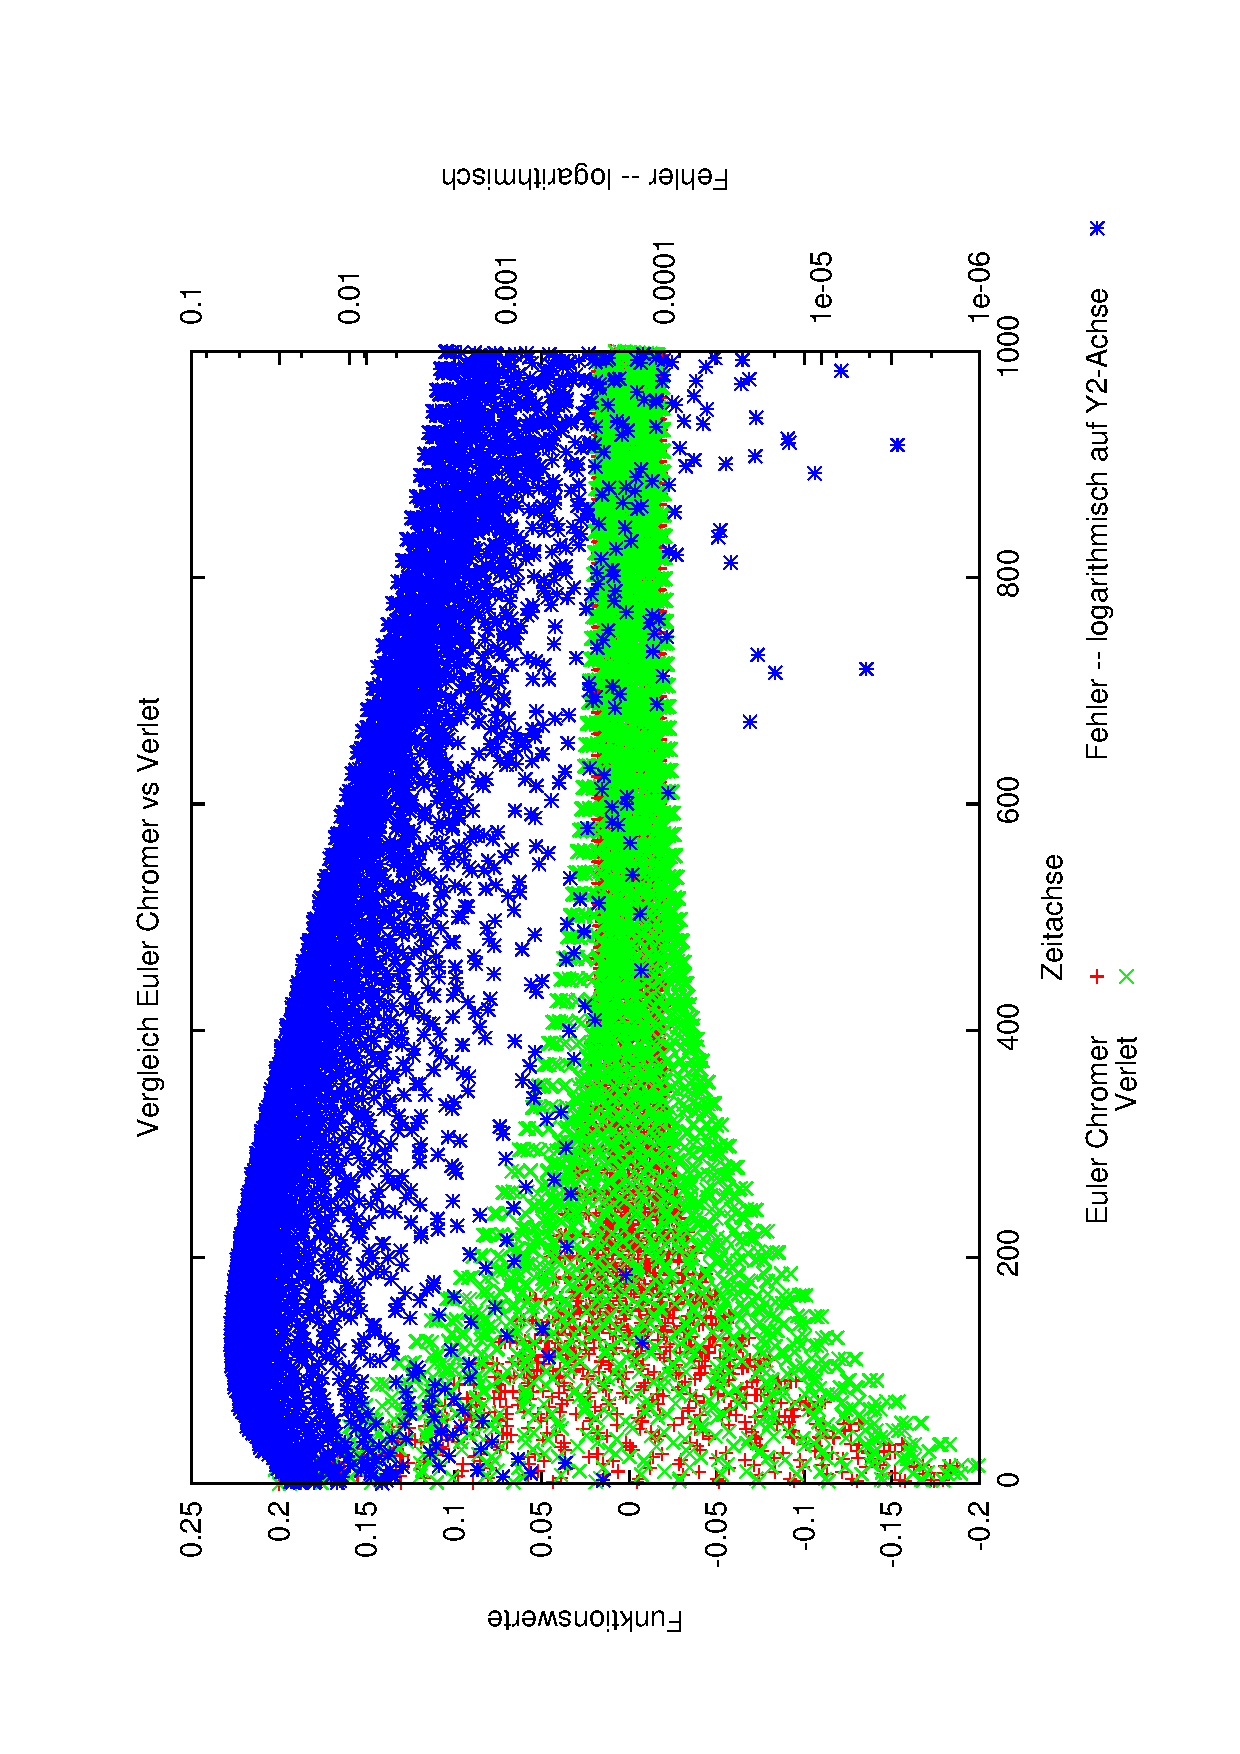
\includegraphics[width=\textwidth]{vgl-euler-1}
  \caption{Vergleich von Euler und Verlet-Verfahren}
  \label{fig:euler-verlet}
\end{figure}

\begin{figure}
  \centering
  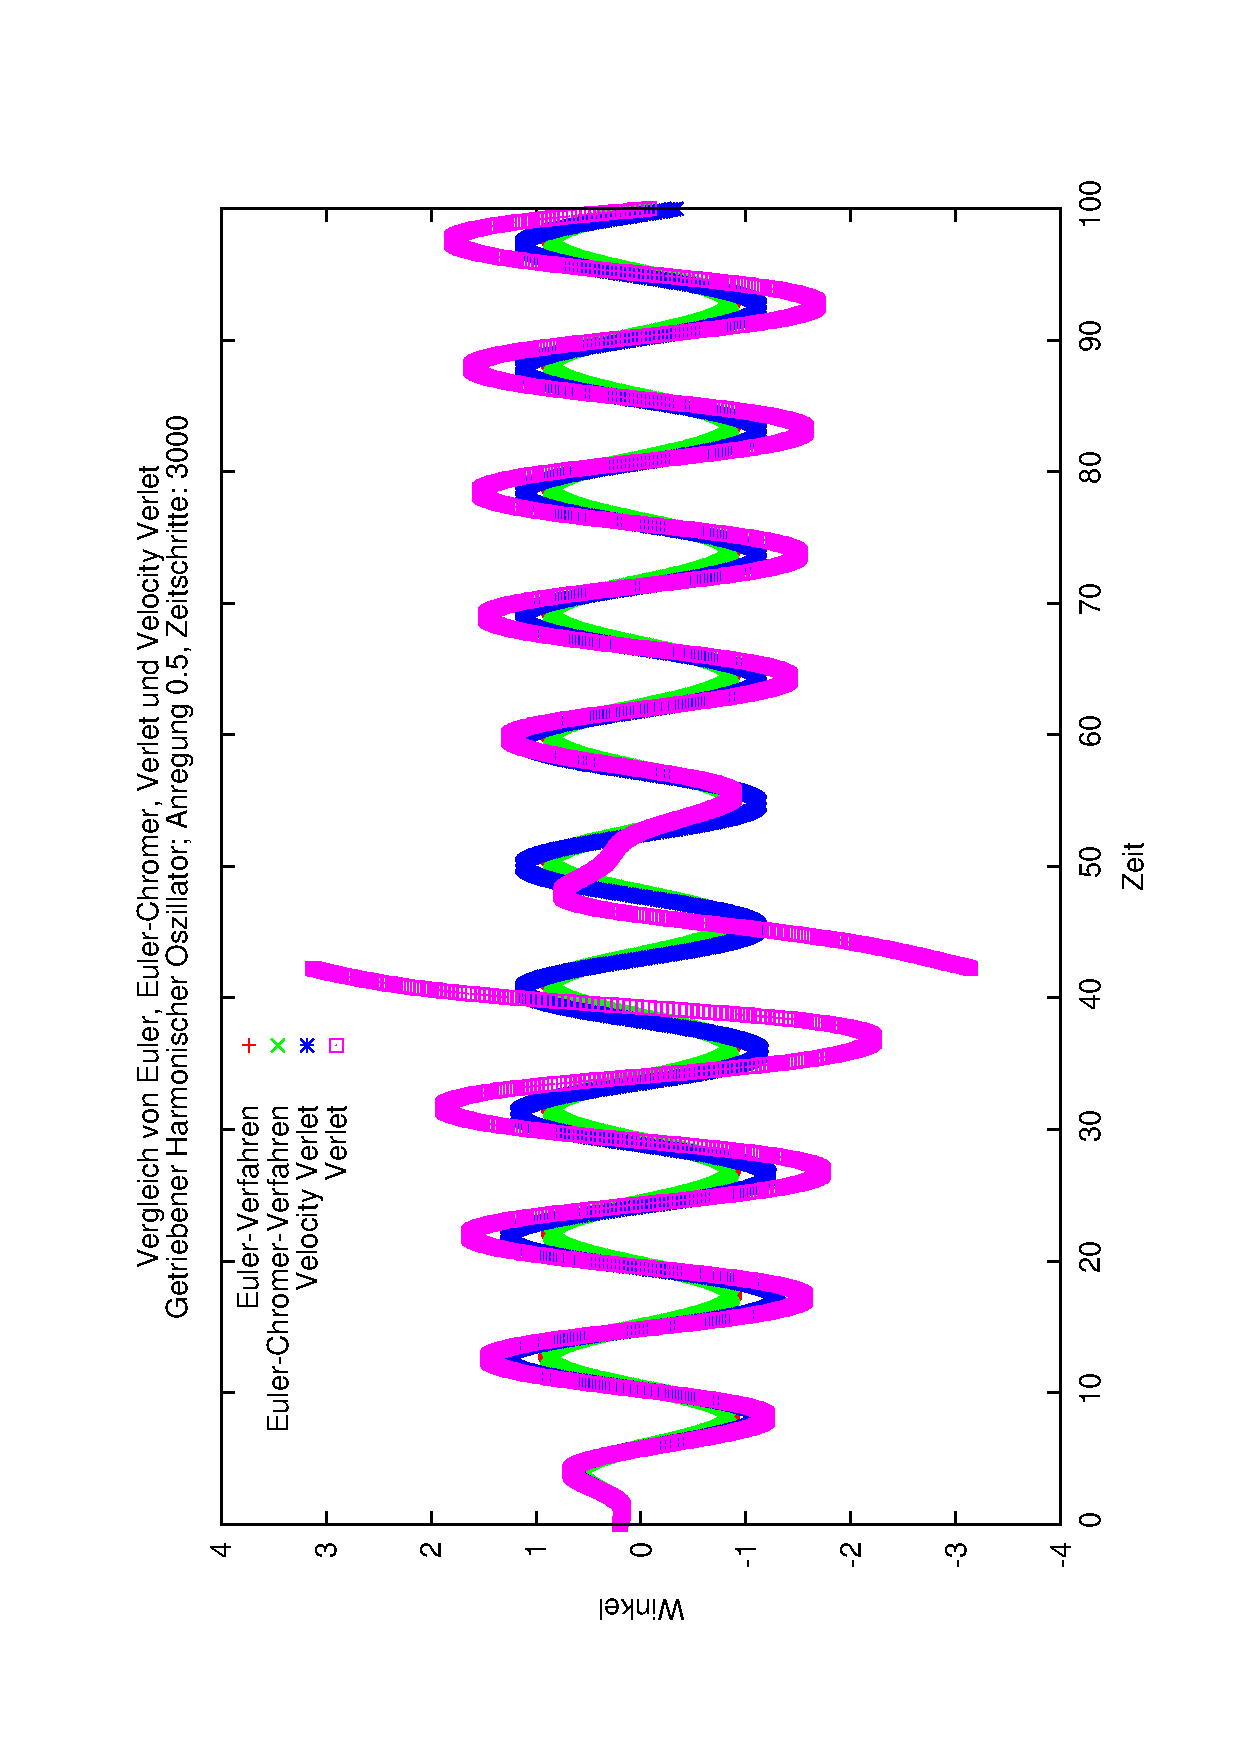
\includegraphics[width=\textwidth]{vgl-awp-3}
  \caption{Vergleich der vier Verfahren f"ur den getriebenen
    Oszillator bei schwachem Antrieb}
  \label{fig:vgl-awp-1}
\end{figure}

\begin{figure}
  \centering
  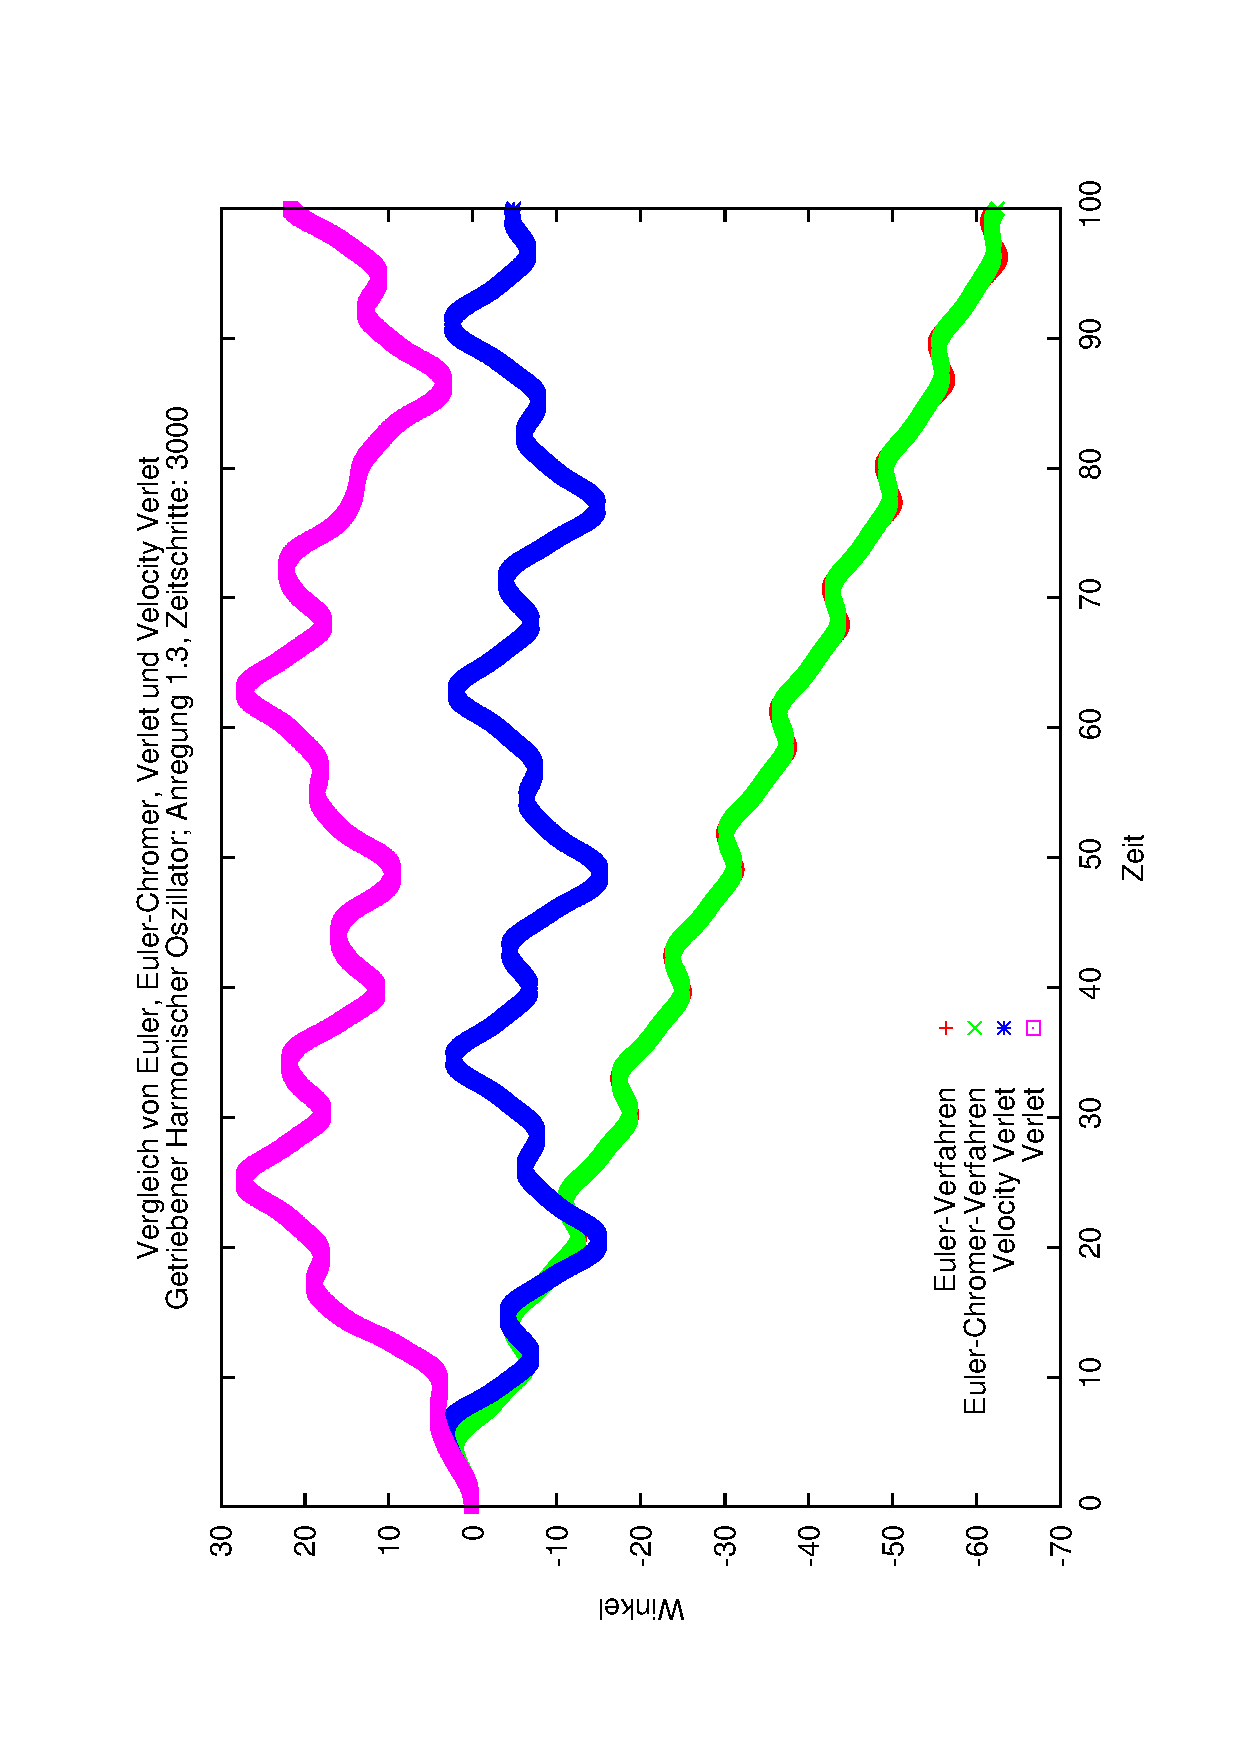
\includegraphics[width=\textwidth]{vgl-awp-1}
  \caption{Vergleich der vier Verfahren f"ur den getriebenen
    Oszillator bei starkem Antrieb}
  \label{fig:vgl-awp-2}
\end{figure}
 
 
 
 

\paragraph{Aufgabe 2: Dynamik einer Federkette}
\label{sec:aufgabe_2:_dynamik_einer_federkette}

Die von mir verwendetet Bewegungsgleichung basiert basiert auf
folgender "Uberlegung. Seien $x_1$, $x_2$ und $x_3$ die Auslenkungen
der Massen aus ihrern Ruhelagen und $D_a$ die Federh"arte der ersten
Feder (zwischen Wand und $x_1$) und entspr. weiter $D_b$, $D_c$ und
$D_d$ definiert, dann erf"ahrt die erste Masse $x_1$ nach
\textsc{Hook} die Kraft
\begin{equation}
  \label{eq:1}
 F_1 =  \underbrace{ -D_a x_1 }_\text{ Von Feder $D_a$ } +
 \underbrace{ D_b x_2
    - D_b x_1 }_\text{ Von Feder $D_b$ } \;.
\end{equation}

Berechnet man analog die Kr"afte auf die zweite und dritte Masse so
kann man dies zusammenfassen:
\begin{align}
  \label{eq:2}
  F_1 = m_1 \ddot x_1 &= -(D_b+D_a) x_1 + D_b x_2 \;, \\
  F_2 = m_2 \ddot x_2 &= D_b x_1 - (D_b+D_c)x_2 + D_dx_3 \;, \\
  F_3 = m_3 \ddot x_3 &= -(D_c + D_d)x_3 + D_c x_2 \;.
\end{align}

Um die Bewegung elegant zu notieren, verwende ich den Vektor
\begin{equation}
  \label{eq:3}
  \vec \xi = (x_1, \dot x_1, x_2, \dot x_2, x_3 , \dot x_3 )^T \;,
\end{equation}
dessen Ableitung
\begin{equation}
  \label{eq:4}
  \dot{ \vec \xi } = ( \dot x_1, \frac{F_1}{m_1},  \dot x_2,
    \frac{F_2}{m_2},  \dot x_3, \frac{F_3}{m_3} )^T
\end{equation}
Eine Funktion von $\dot x_i$ und $F_i$ ist, wopbei man die $F_i$ durch
die $x_i$ ausdr"ucken kann. Es ist also
\begin{equation}
  \label{eq:5}
  \dot{ \vec \xi } = f( \vec \xi ) \;,
\end{equation}
und diese DGL kann man mit Runge-Kutta integrieren.

Um den Vektor $\vec \xi$ auch im Programm zu verwenden, habe ich die
Vektorklasse $\texttt{Vector6D.h}$ angepasst. Die Implementierung ist
in \texttt{federn01.cpp} und die Ausgabe mit den Anfangsbedingungen
\begin{equation}
  \label{eq:6}
  \vec \xi_0 = ( 0., 0., 0., 0., 1.1/12., 0. )
\end{equation}
ist f"ur $t \in [ 0 , 10 ]$ mit 500 Zeitschritten in
Abb. \ref{fig:federn01} dargestellt.

Was auff"allt ist, dass sich die Trajektorien "uberschneiden -- das
ist nat"urlich nicht sinnvoll, weil sich in Realit"at die Massen nicht
durchdringen k"onnen, au"serdem gilt das \textsc{Hook}'sche Gesetz
nicht unbedingt -- es ist f"ur realie Feder nur eine N"aherung.

\begin{figure}
  \centering
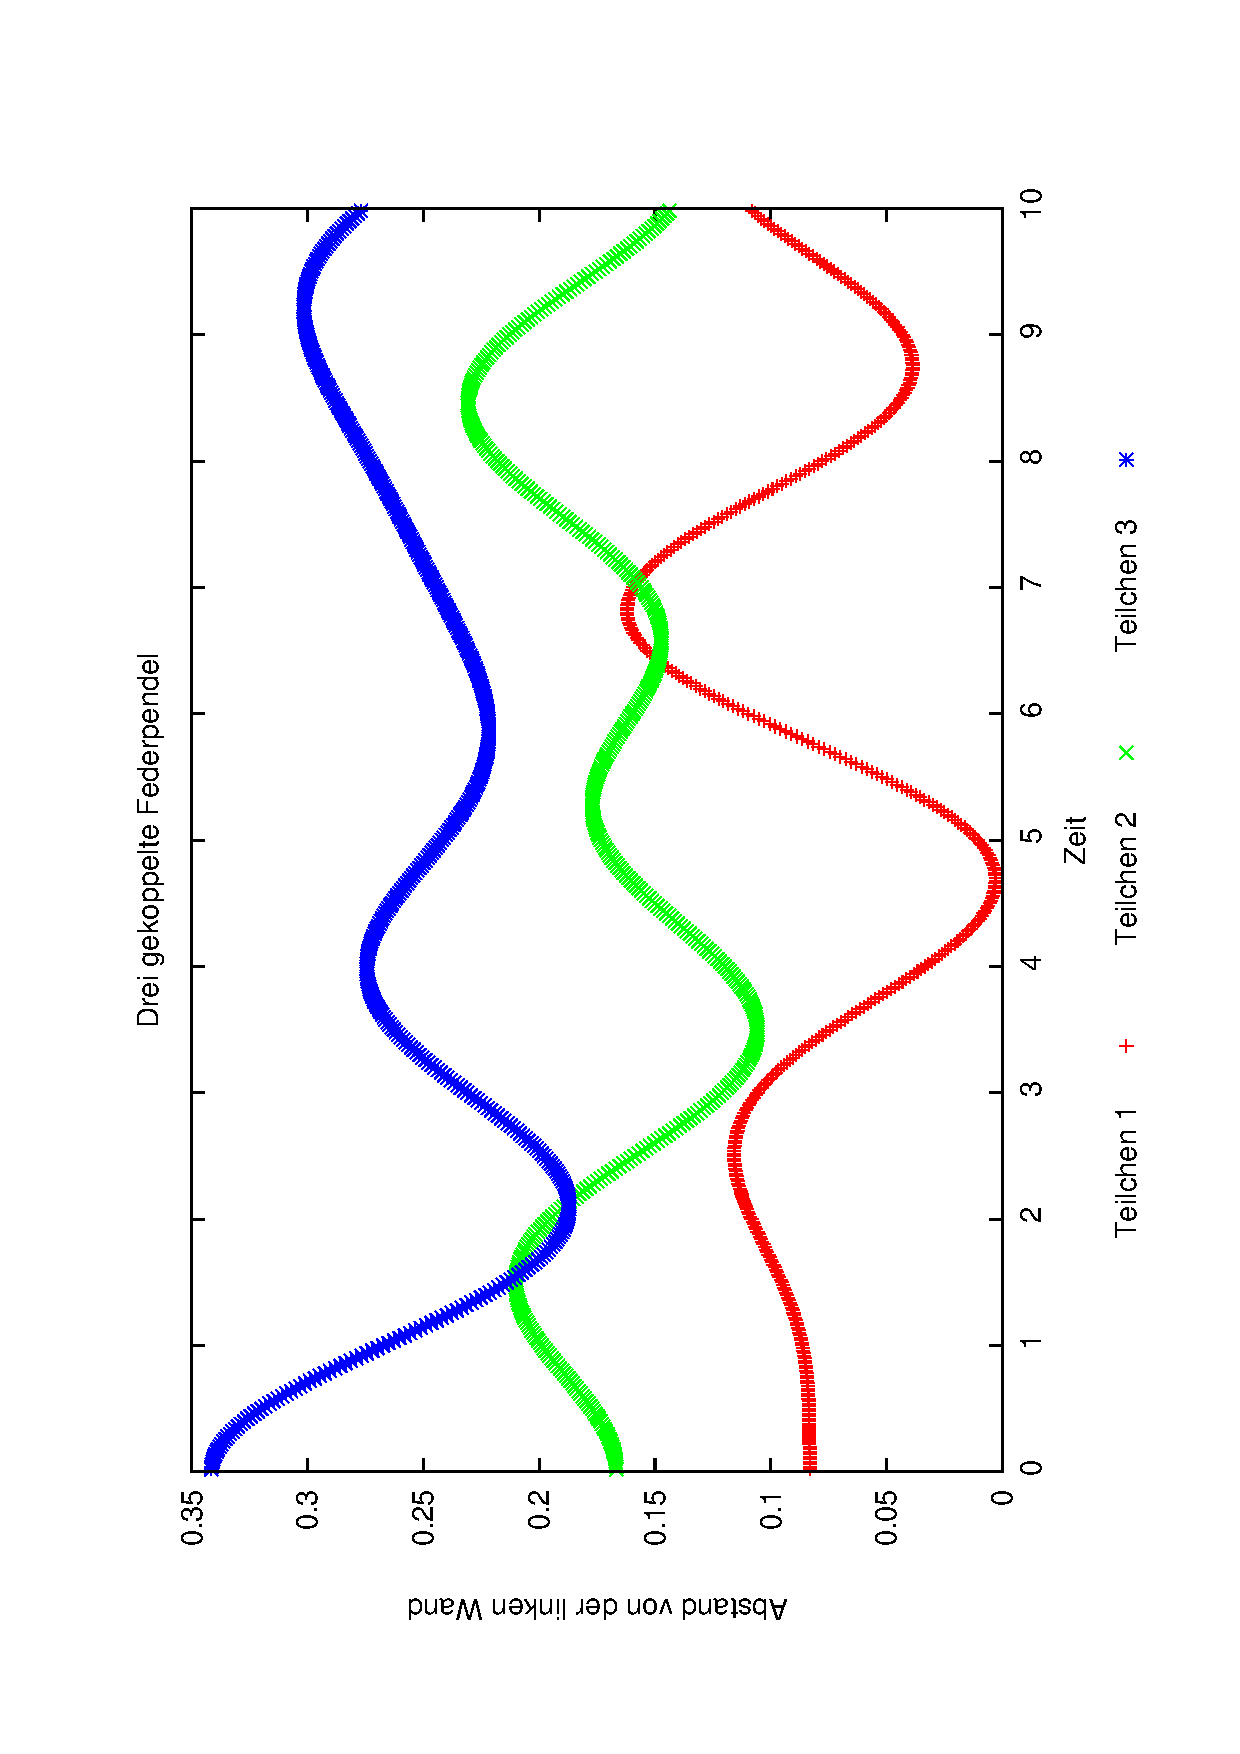
\includegraphics[width=\textwidth]{tranjektorie-federn01-1}
  \caption{Drei durch Federn gekoppelte Massen, 500 Zeitschritte}
  \label{fig:federn01}
\end{figure}
 
In Abb. \ref{fig:vgl-schritte} sind die selben Anfangsbedingungen f"ur
verschiedenen Anzahlen von Zeitschritten ($N$) aufgetragen. Hier sieht
man, dass auch f"ur gro"se Zeitschritte ($10/N$; also kleine $N$) das
Verfahren noch sehr genau ist; sogar bei $N=20$ -- also f"ur nur 2
Zeitschritte pro Zeiteinheit -- erkennt man noch die characteristische Bewegung.

\begin{figure}
  \centering
  \subfigure[$N =
  1000$]{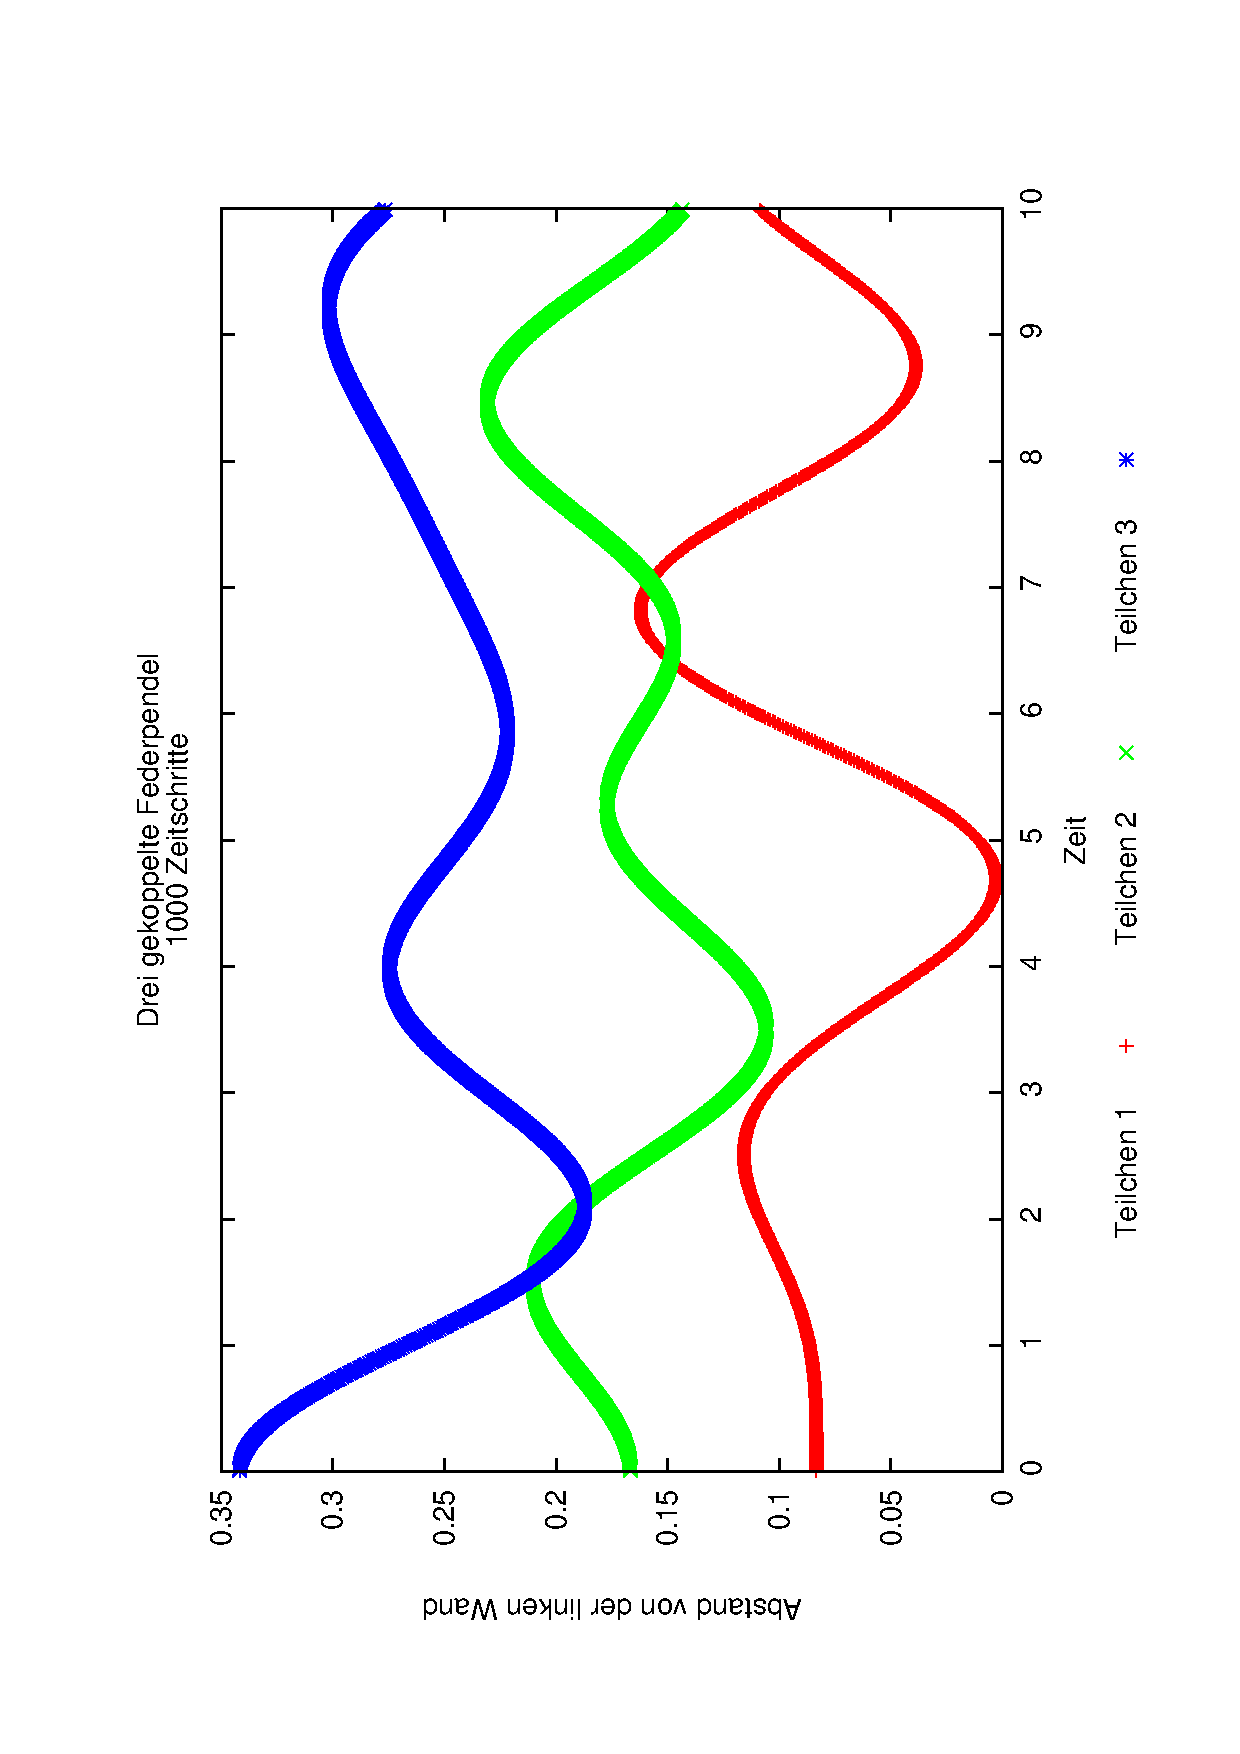
\includegraphics[width=0.3\textwidth]{tranjektorie-federn01-6}}
\subfigure[$N =
  500$]{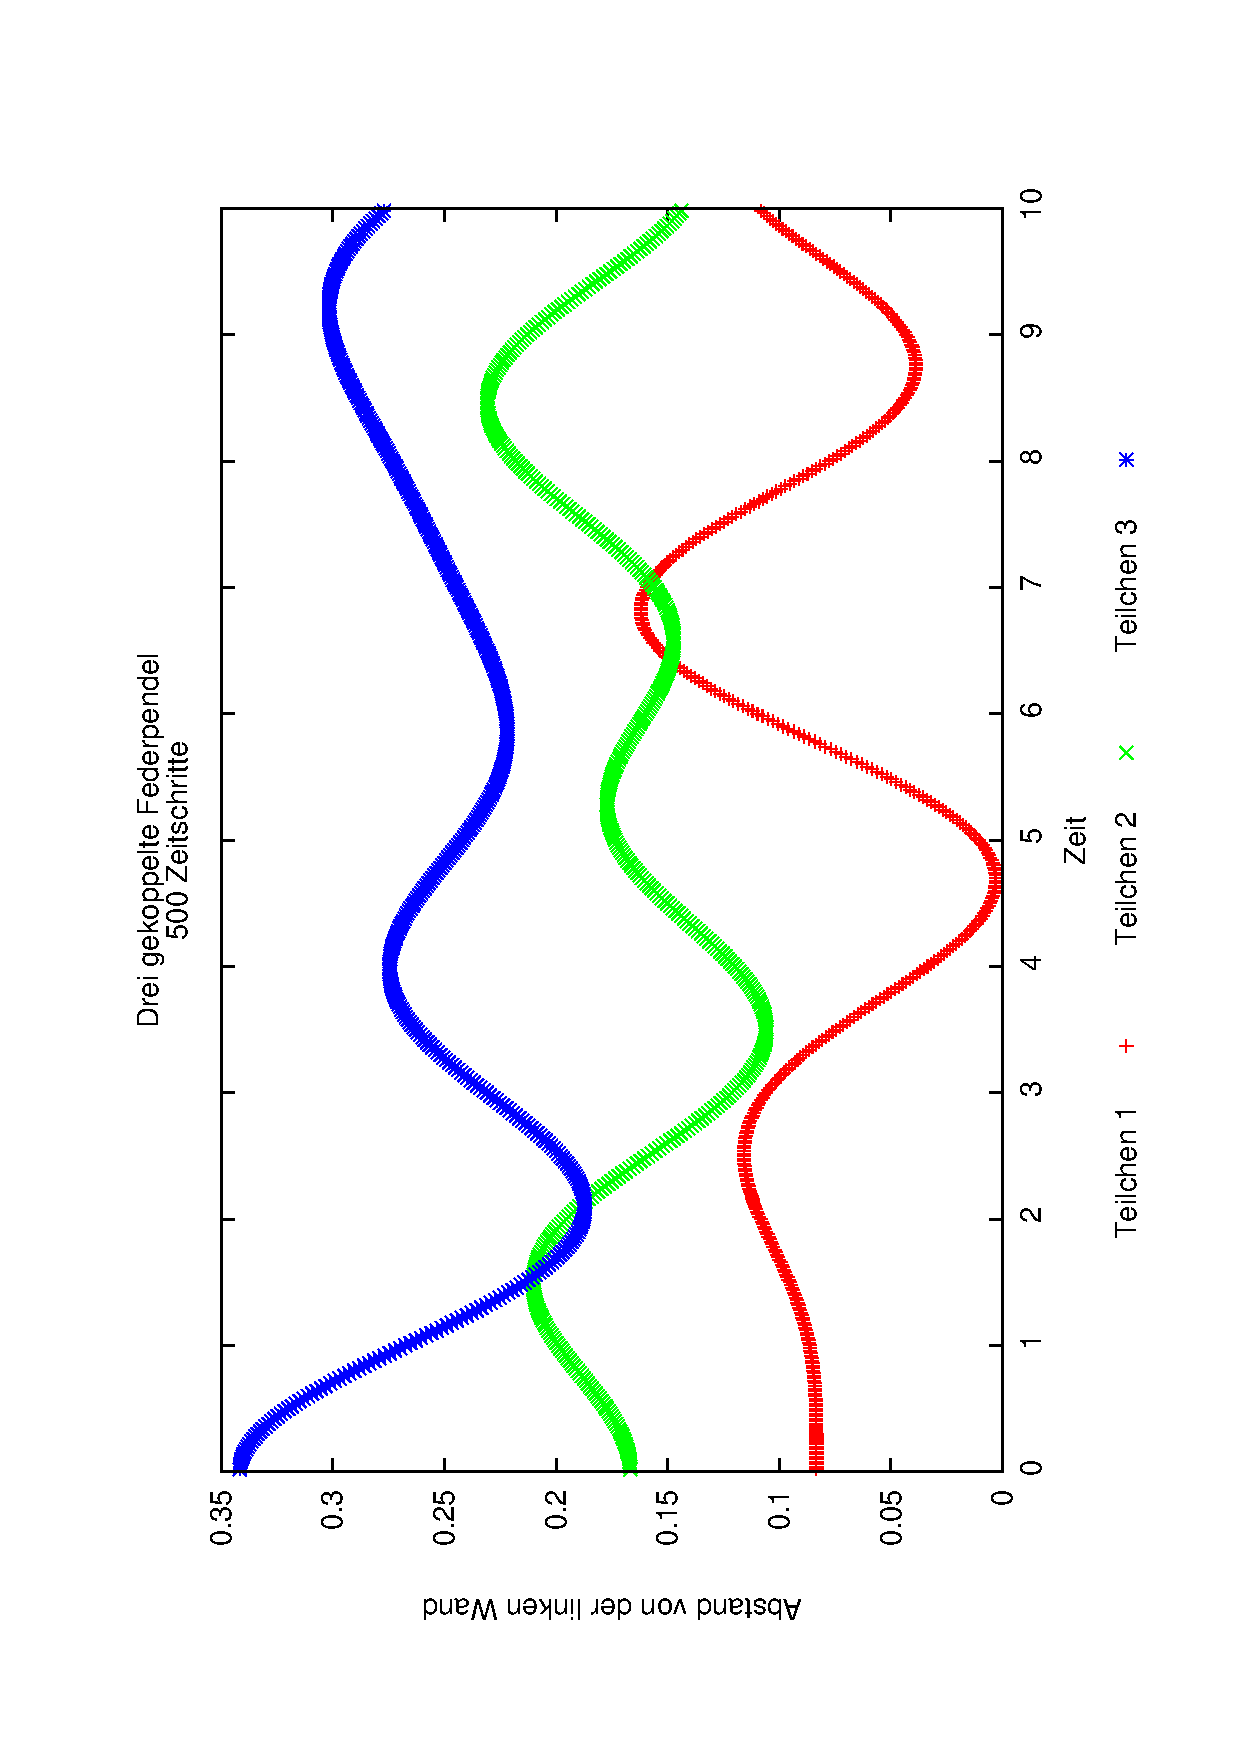
\includegraphics[width=0.3\textwidth]{tranjektorie-federn01-2}}
  \subfigure[$N =
  50$]{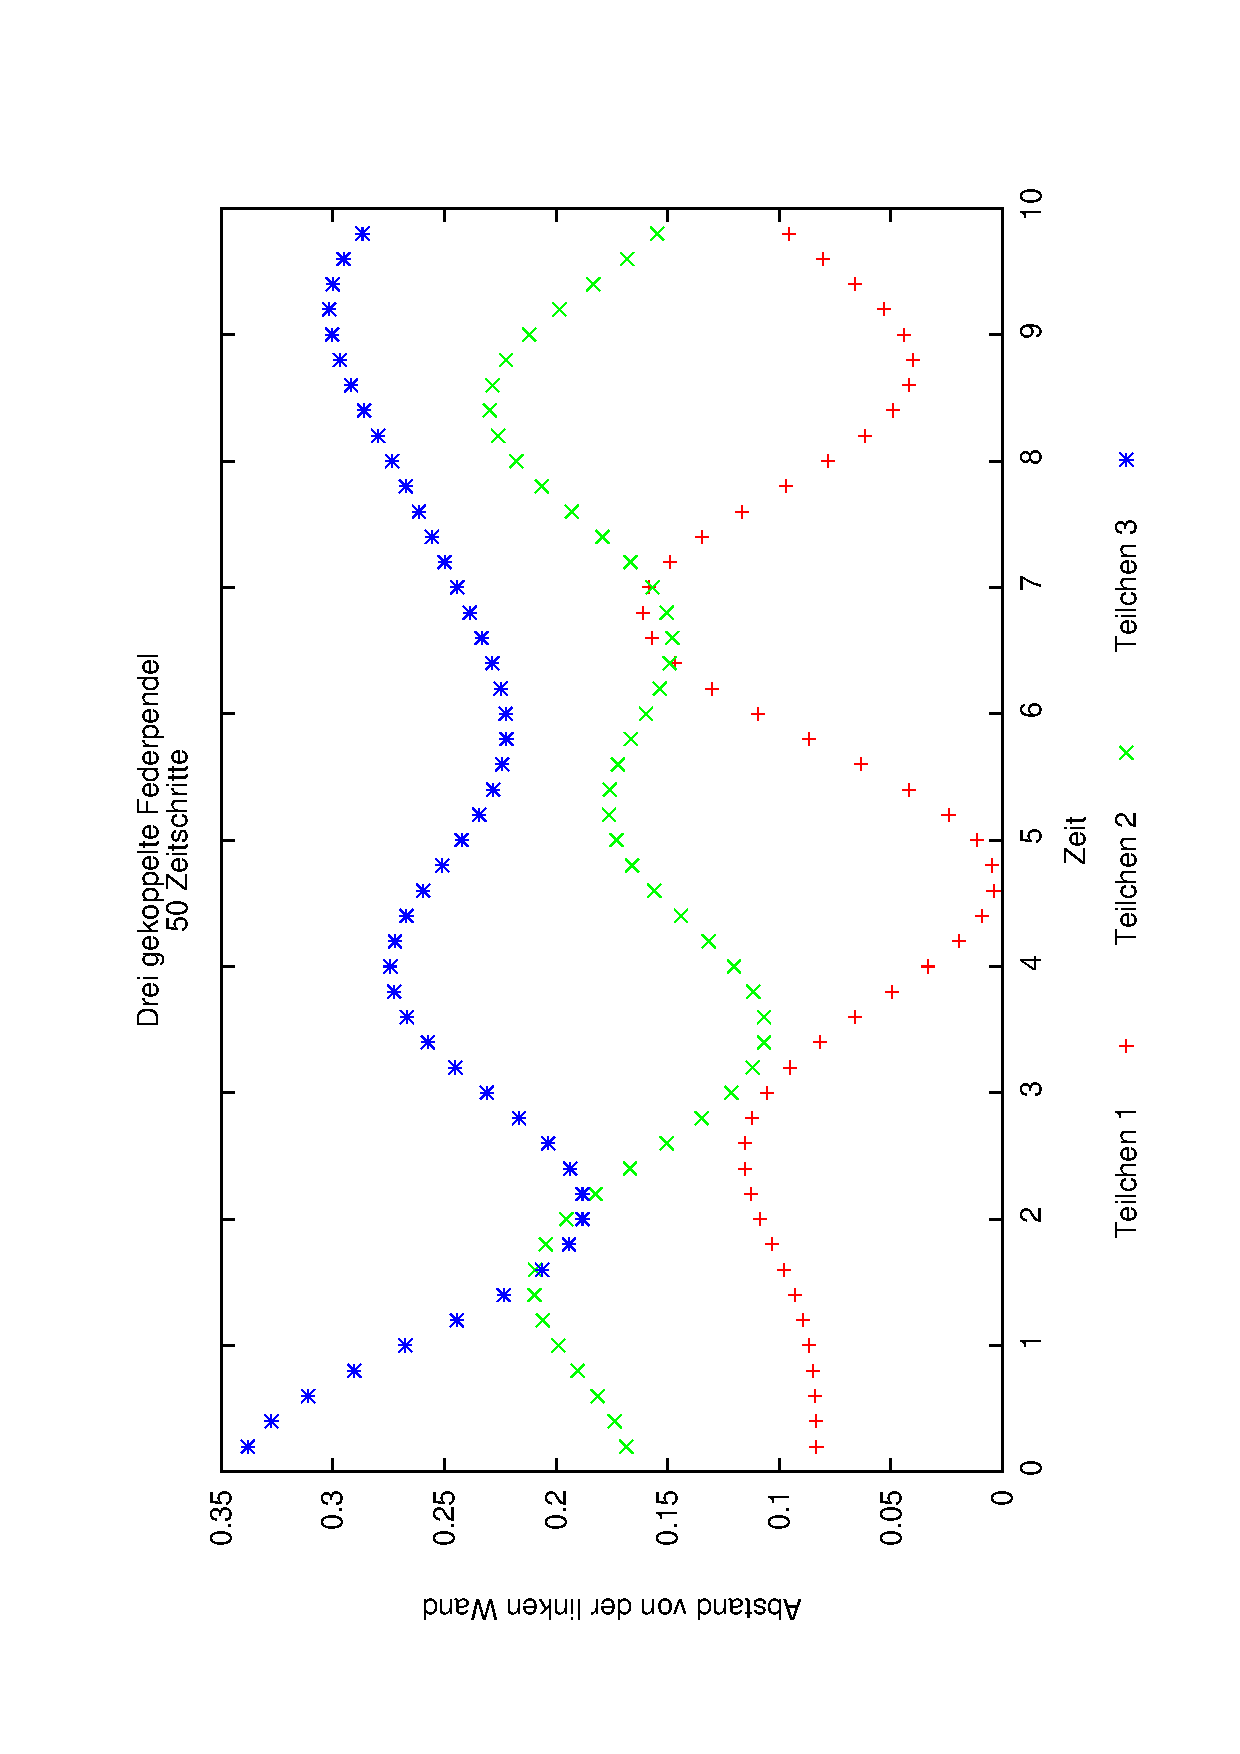
\includegraphics[width=0.3\textwidth]{tranjektorie-federn01-3}}
  \subfigure[$N =
  30$]{\includegraphics[width=0.3\textwidth]{tranjektorie-federn01-4}}
  \subfigure[$N =
  20$]{\includegraphics[width=0.3\textwidth]{tranjektorie-federn01-5}}
  \subfigure[$N =
  10$]{\includegraphics[width=0.3\textwidth]{tranjektorie-federn01-7}}
  \caption{Gekoppelte Pendel mit verschieden gro"sen Zeitschritten}
  \label{fig:vgl-schritte}
\end{figure}






\paragraph{Populationsdynamik: Volterra- und Lotka-Volterra-Modell}
\label{sec:popul_volt_und_lotka_volt}

Die Implementierung zu beiden Verfahren findet sich in
\texttt{population01.cpp}.

In Abb \ref{fig:volterra} sind f"ur die drei angegebenen
Anfangsbedingungen (es ist jeweils $m = 0.2$ und $b = 0.1$)
characteristische Zeiten geplottet.

\begin{figure}
  \centering
  \subfigure[$y(0) = (0.25,
  0.25)^T$]{\includegraphics[width=0.3\textwidth]{volterra_025-025}\label{volterra-klein}}
  \subfigure[$y(0) = (0.5,
  0.5)^T$]{\includegraphics[width=0.3\textwidth]{volterra_050-050}}
  \subfigure[$y(0) = (1.0 ,
  1.0)^T$]{\includegraphics[width=0.3\textwidth]{volterra_100-100}}
  \caption{Volterra}
  \label{fig:volterra}
\end{figure}

\begin{itemize}
\item F"ur $y(0) = (0.25,  0.25)^T$ ergibt sich eine Periodendauer von
  $50$ und eine Amplitude von $(0.4 , 0.26)^T$, 
\item f"ur $y(0) = (0.5,  0.5)^T$ eine Periodendauer von $75$ und eine
  Amplitude von $(0.85 , 0.65)^T$ und
\item f"ur $y(0) = (1.0 , 1.0)^T$ eine Periodendauer von $100$ und
  eine Amplitude von $(1.8 , 1.5)$.
\end{itemize}
 
\abs Das Volterra-Modell zeigt ein periodisches Gleichgewicht. Dies
kann die Natur wohl sehr gut beschreiben; bspw sieht die Schneehasen-
und Schneefuchspopulation oder die Sardienenpopulation im Mittelmeeh
in ihrer zeitlichen Entwicklung dem ziemlich "ahnlich. Deswegen ist
diese Modell grunds"atzlich geeignet.

\abs
Erg"anzt man das Modell zum Lotka-Volterra-Modell, ber"ucksichtigt man
die beschr"ankte Kapazit"at eines Gebiets, Lebewesen zu unterhalten.

In Abb. \ref{fig:phasen} sieht man -- dies sind Phasendiagramme --,
dass sich bei einer verh"altnism"a"sig gro"sen Schranke die
Populationen nicht sonderlich von dem Volterra-Modell unterscheiden,
weil das Gebiet sehr viele B"autetiere unterhalte kann, sodass dies
wegen ihrer nat"urlichen Dezimierung nur selten an die Grenzen
kommen. Erst bei kleinen Schranken sieht man einen deutlichen Effekt:
Die Phasentrajektorie l"auft auf einen Fixpunkt zu; dort wird sich ein
statisches -- und stabiles -- Gleichgewicht der beiden Populationen
bilden.

In Abb.~\ref{fig:lotka} sieht man dazu noch die Zeitentwicklung. F"ur
die kleine Schranke kann man schon sehen, wie sich ein statisches
Gleichgewicht einstellt, wohingegen sich Abb. \ref{lotka-gross} nur
wenig von Abb. \ref{volterra-klein} unterscheidet.\footnote{Beachte
  verschiedene Zeitscalen!}

\begin{figure}
  \centering
  \subfigure[Sehr kleine
  Schranke]{\includegraphics[width=0.45\textwidth]{phase_025-025-005}}
  \subfigure[Gro"se
  Schranke]{\includegraphics[width=0.45\textwidth]{phase_025-025-005}}
  \caption{Phasendiagramme der Modelle im Vergleich}
  \label{fig:phasen}
\end{figure}
 
\begin{figure}
  \centering
  \subfigure[Sehr kleine
  Schranke]{\includegraphics[width=0.45\textwidth]{lotka_025-025-005}}
  \subfigure[Gro"se
  Schranke]{\includegraphics[width=0.45\textwidth]{lotka_025-025-100}\label{lotka-gross}}
  \caption{Zeitdiagramme des Lotka-Volterra-Modells}
  \label{fig:lotka}
\end{figure}




\end{document}














%%% Local Variables: 
%%% mode: latex
%%% TeX-master: t
%%% End: 
